%% chapter 3 Land use and functional diversity

\section*{Keywords}
Land use; land-use intensity; terrestrial vertebrates; functional diversity; traits.

\section*{Abstract}
Land-use change is the leading driver of global biodiversity loss, thus characterising its impacts on the functional structure of ecological communities is an urgent challenge. Using a database describing vertebrate assemblages in different land uses, I assess how the type and intensity of land use affect the functional diversity of vertebrates globally. I find that human land uses alter local functional structure by driving declines in functional diversity, with the strongest effects in the most disturbed land uses (intensely used urban sites, cropland and pastures), and among amphibians and birds. Both tropical and temperate areas experience important functional losses, which are only partially offset by functional gains. Tropical assemblages are more likely to show decreases in functional diversity that exceed those expected from species loss alone. These results indicate that land-use change non-randomly reshapes the functional structure of vertebrate assemblages, raising concerns about the continuation of ecological processes sustained by vertebrates.

\section{Introduction}
Anthropogenic activities are profoundly transforming global biodiversity. Although multiple pressures act in combination, land-use change currently poses the greatest threat to biodiversity \citep{Maxwell2016, Newbold2015}. However, not all species respond similarly to land-use change. Traits have been found to explain species' sensitivity to land-use change in diverse groups \citep{Newbold2013, Nowakowski2017, Quesnelle2014, Todd2017}. Previous work has also shown that land-use change leads to non-random modification of assemblage trait composition (or functional diversity) \citep{Chapman2018, Colin2018, Flynn2009, LaSorte2018, Newbold2013, Tinoco2018}. Since it is widely acknowledged that biodiversity, and in particular trait diversity, may promote ecosystem functioning and stability, modification to the trait composition of assemblages could have far-reaching and adverse impacts on ecological processes \citep{Hooper2012, Magioli2021, Oliver2015, Tilman1994}.

Terrestrial vertebrates support many processes, ranging from pollination \citep{Ratto2018}, to seed dispersal to the regulation of lower trophic levels \citep{Barber2010, Letnic2012, Salo2010,Zhang2018}. However, we lack a global understanding of how the functional diversity of entire vertebrate assemblages responds to changes in land use. Most previous studies have been conducted at regional or local scales \citep{Davison2021}, but these may not be representative of global patterns. Indeed, recent global syntheses have highlighted how biodiversity responses can differ substantially between regions and across latitudes, with higher sensitivity reported for the tropics \citep{Matuoka2020,Millard2021, Newbold2020}. Another key issue is the taxonomic coverage of past work. Few studies investigating effects of land use on functional diversity have considered several vertebrate classes together, and comparative studies remain rare. Thus, how land-use change affects the functional diversity of local vertebrate assemblages at global scales, and the potential geographical and taxonomic variation in the effects, still largely remains to be explored.

Here, I aim to assess how human land use and land-use intensity affect the functional diversity of vertebrate assemblages, across and within taxonomic classes. Building on recent work \citep{Matuoka2020,Millard2021, Newbold2020}, I investigate differences in response between tropical and temperate regions. I use multiple response metrics to quantify functional diversity. First, functional richness measures the breadth and variety of trait combinations represented in an assemblage \citep{Legras2018}. Second, functional dispersion quantifies how similar species in a given assemblage are in terms of their traits \citep{Laliberte2010}. These metrics can mask important alterations of assemblage composition if functional losses are compensated for by functional gains. To address this, I consider pairwise measures between assemblages, to explore levels of functional loss and functional gain across land uses (Figure \ref{chap3_fig1}).

%% Figure 1 %%

%%%%%%%%%%%%%%

To this end, I combine (1) the trait data across terrestrial vertebrates collected in Chapter 2 with (2) global records of species occurrence in eight land-use types of differing intensity of use (the PREDICTS database: \citet{Hudson2014, Hudson2017}; Figure \ref{chap3_fig1}; Appendix 2, Table \ref{SI3_Table1}). The PREDICTS database is currently the most comprehensive database of sampled species occurrence, and for most records also abundance, across multiple land uses of different land-use intensity. Using the PREDICTS database allows me to contrast biodiversity metrics among intact land uses (primary-vegetation sites, considered to be the undisturbed reference condition), and all other human land-use types. Specifically, I test the following hypotheses, both across and within taxonomic classes:

\begin{enumerate}
\item I expect decreases in functional diversity in human land uses compared to primary vegetation, caused by contractions of occupied trait space. I expect such effects to be more pronounced where land is used more intensively by humans. This hypothesis builds upon evidence that species with certain traits are more sensitive to land-use disturbance \citep{Newbold2013}, meaning that disturbed land uses will retain only disturbance-tolerant species, more functionally similar to one another. Given the reported higher sensitivity of tropical assemblages to land-use disturbance, I predict that such effects are stronger in the tropics.
\item I hypothesise that decreases in functional diversity in disturbed land uses exceed decreases expected by chance, given local species loss. Thus, I expect disturbed land uses to promote functional under-dispersion. Functional under-dispersion occurs when species within an assemblage are more similar, in term of their traits, than expected by chance \citep{Cadotte2017, Wong2018} -- or, in other words, when functional dispersion is lower than expected given local species richness. I predict that under-dispersion is more likely to occur in the highly disturbed sites, in both temperate and tropical areas. This hypothesis is based on the idea that species are being removed non-randomly from sensitive areas of the trait space, and increasingly so with higher disturbance level.
\item Finally, I expect decreases in functional diversity in human land uses to be driven by high functional loss, whereby species are being removed from previously occupied areas of the trait space; I expect no functional gain. This hypothesis is based on the idea that the functional trait space in undisturbed land uses represents all of the possible regional trait combinations and that species with functional attributes rendering them unable to persist in altered conditions will be filtered out \citep{Cornwell2006}.
\end{enumerate}

%% figure 1 - overview of study design and functional metrics
\begin{figure}[h!]
\centering
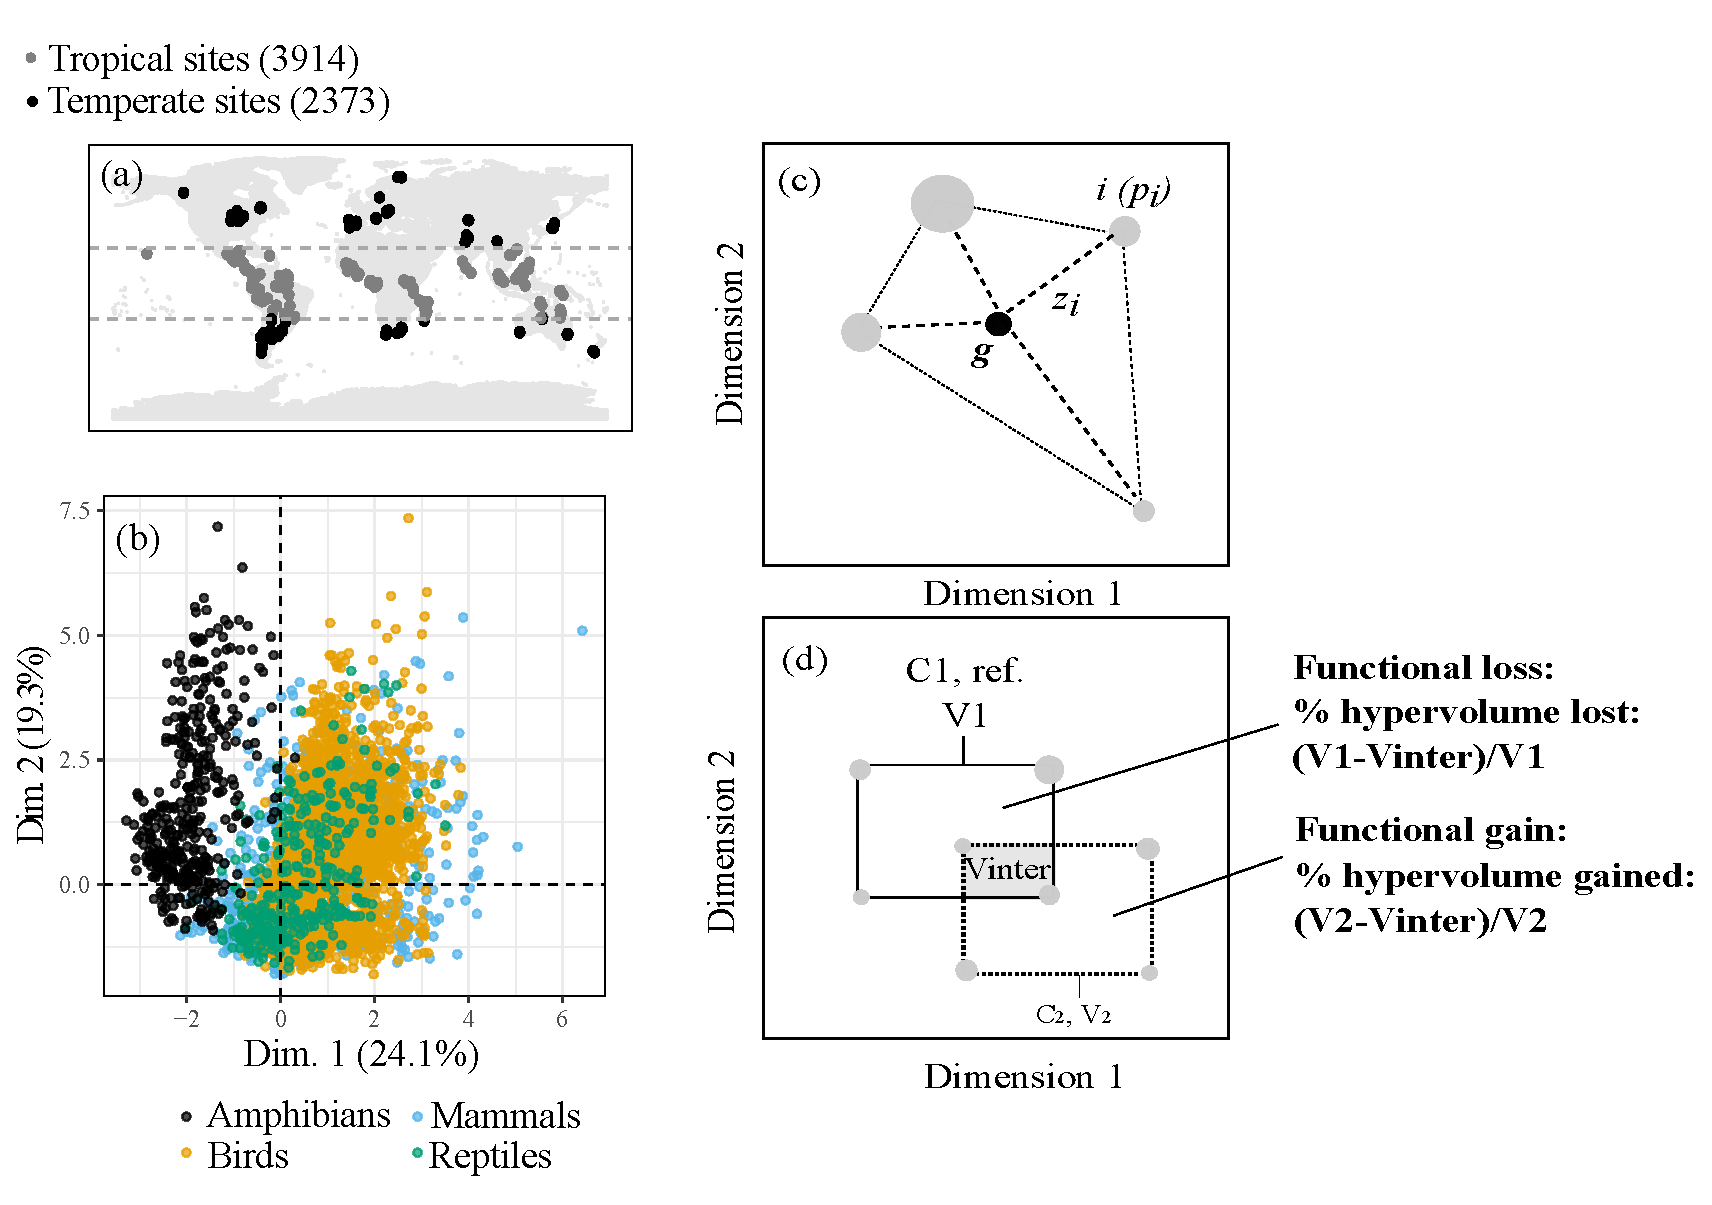
\includegraphics[scale=0.55]{figures/Chapter_FD/Figure1}
\caption[Overview of the study design and functional diversity metrics]{\textbf{Overview of the study design and functional diversity metrics.} I used occurrence data for vertebrate species from the PREDICTS database (\citep{Hudson2014, Hudson2017}; 180 studies; 431,170 records; 4,339 species; 6,758 sampled sites). \textbf{(a)} shows the spatial distribution of sites I consider. I combine occurrence data with trait data compiled in Chapter 2 to calculate functional diversity metrics. \textbf{(b)} is a representation of the trait data in two dimensions, plotted across PREDICTS vertebrates. Traits that contributed most to dimension 1 were lifespan (29\%) and litter/clutch size (22\%), while traits that contributed most to dimension 2 were habitat breadth (47\%) and use of artificial habitats (35\%). \textbf{(c)} and \textbf{(d)} present the conceptual framework for the calculation of the functional diversity metrics: local measures (c) and pairwise metrics (d). \textbf{(c)} Given a trait space, functional richness is calculated as the hypervolume occupied by the minimum convex hull encompassing all species \citep{Villeger2008}. Functional dispersion is calculated as the mean distance of the species to the centroid, \textbf{\textit{g}} \citep{Laliberte2010}. \textbf{(d)} I compute functional loss as the proportion of hypervolume lost from the reference assemblage, and I define functional gain as the proportion of hypervolume of the disturbed assemblage that was gained (proportion of novel trait space in the disturbed assemblage). \textit{Figure reproduced from \citet{Etard2021}.}}
\label{chap3_fig1}
\end{figure}



\section{Methods}

\subsection{Vertebrate assemblages}

I used vertebrate occurrence data from the PREDICTS database \citep{Hudson2014, Hudson2017}, a collection of studies that recorded species occurrence across multiple land uses and land-use intensities. In PREDICTS, each study contains several sites, which may be clustered into spatial blocks. Assemblage and land-use data are available at the site level: one site is characterised by a unique land use of given land-use intensity and provides occurrence data for a set of sampled taxa (and the same set of taxa is sought at all other sites within a study). Sites located between 23.5$^{\circ}$N and 23.5$^{\circ}$S of latitude were considered tropical, and otherwise temperate (Figure \ref{chap3_fig1}).

Land uses in PREDICTS were assigned to the following categories, based on the descriptions of the habitat given by the original collectors of the data: primary vegetation (considered to be the undisturbed reference); secondary vegetation; plantation forest; pasture; cropland; urban (considered human, or disturbed; Appendix 2, Table \ref{SI3_Table1};  \cite{Hudson2014, Hudson2017}). Secondary vegetation is further divided into three categories: mature, intermediate and young, depending on the stage of recovery of the vegetation. Land-use intensity is reported as minimal, light or intense, according to criteria that depended on the land-use type in question (e.g., crop diversity, degree of mechanisation and chemical inputs in cropland, or bushmeat harvesting and selective logging in primary vegetation; \cite{Hudson2014}). I excluded sites for which the land use could not be characterised or for which the stage of recovery of secondary vegetation was unclear. As the PREDICTS database is a collection of independent studies, the design of this study was not balanced: the sample size varied across land uses (Appendix 2, Figures \ref{SI3_F1} \& \ref{SI3_F2}), and across taxonomic groups (3,103 species of birds; 531 mammals; 379 amphibians; 326 reptiles).

\subsection{Functional traits and diversity metrics}
Trait choice is a critical step when calculating functional diversity metrics, which are highly sensitive to trait selection \citep{Mouillot2021}. However, trait selection trades off with data availability. Here, a constraint was to use similar traits across the different classes. %We chose seven traits from a compilation across terrestrial vertebrates \citep{Etard2020}, most of which are available for at least 50\% of the species in each class (except trophic level in amphibians and lifespan in herptiles [Figure S4]). 
Thus, I used the seven traits compiled in Chapter 2 across terrestrial vertebrates. Most of these traits were available for at least 50\% of the species in each class (except trophic level in amphibians and lifespan in herptiles; Appendix 2, Figure \ref{SI3_F4}). In addition, I chose traits that were ecologically relevant, broadening the biological definition of traits (i.e., a characteristic measurable at the level of an individual) to include measures of habitat breadth and habitat specialisation (still theoretically measurable at the level of an individual).  The final set constituted seven traits that influence species' responses to environmental change: body mass, trophic level, lifespan, litter/clutch size, diel activity, habitat breadth and use of artificial habitats. These traits related to life-history, habitat specialisation and use of geographical space (e.g., habitat breadth significantly explains geographical range size in all classes; Appendix 2, Figure \ref{SI3_F3}). Here, I did not consider estimations of dispersal abilities or home range size as these were available for a small fraction of the species ($<$3\%, \cite{AlexSmith2005, Paradis1998, Sutherland2000, Whitmee2013a}), neither did I include geographical range size which is measured across many individuals, and hence cannot be considered a trait. As in Chapter 2, I did not consider intraspecific trait variation, thus assuming no effect of the environment on trait values.

Trait coverage was variable among classes and traits, with important gaps for reptiles and amphibians (Appendix 2, Figures \ref{SI3_F4} \& \ref{SI3_F5}; Chapter 2). I imputed missing trait values using random forest algorithms (`missForest' package: \citet{Stekhoven2012}, \citet{Stekhoven2016}), including traits, taxonomic order and phylogenetic eigenvectors as predictors \citep{Debastiani2021, Penone2014}. To further assess the sensitivity of the results to imputation (see next section), I imputed missing trait values eight times, thereby obtaining eight sets of imputed traits. I randomly selected one imputed trait set for the calculation of functional metrics. Imputations of missing trait values \& imputation performance are detailed in Appendix 2, S3.2: `Trait data \& imputation of missing trait values' and S3.4: `Imputation performance' (and Figures \ref{SI3_F6}-\ref{SI3_F8}). Post-imputation, continuous traits were log$_{10}$-transformed (except habitat breadth which was square-rooted) and z-scored (standardised to unit variance and zero mean). In addition, I assessed whether the results were robust to imputation error using a subset of the PREDICTS data considering only species for which I had complete trait information (see next section).

Correlation among traits can be a safeguard against high sensitivity of functional metrics to trait omission, notably where omitted traits correlate strongly with traits that are already included in the calculation \citep{Mouillot2021}. Nevertheless, high multicollinearity among traits has been reported as potentially problematic for the calculation of functional diversity \citep{Cadotte2011}. Thus, I verified that the degree of multicollinearity among traits was not problematically high (with a threshold of 5 for variance inflation factors, Appendix 2, Table \ref{SI3_Table3}). Furthermore, I tested the sensitivity of the results to trait omission, by investigating whether adding geographical range size in the calculation of functional metrics was likely to affect the results.


\subsection{Effects of land use and land-use intensity on FRic and FDis (Hypothesis 1)}

For each assemblage, I measured functional richness using `FRic' \citep{Villeger2008}, and functional dispersion using `FDis’ (\citet{Laliberte2010}; Figure \ref{chap3_fig1}), from the `FD' package (\citet{Laliberte2010}; \citet{Laliberte2015}). I assessed the effects of land use, land-use intensity, and region (temperate versus tropical) on FRic and FDis across and within taxonomic classes using linear mixed-effects models (`lme4' package, \citet{Bates2015}). Land use and land-use intensity were not ranked in the models. A random intercept of study identity accounted for variation in experimental design across studies, while a random intercept representing spatial blocks of sampled sites, nested within study, accounted for spatial structuring within studies. To improve normality and bound predictions between 0 and 1, I transformed FRic and FDis using an arcsin-square-root transformation. The best-fitting model was sought using backwards stepwise model selection, starting with the most complex model that included all two-way interactions among the specified main effects. Model fits were compared using likelihood-ratio tests at each iteration of the selection procedure.

Across vertebrates, the starting models included the effects of land use, land-use intensity and region (temperate versus tropical). The best-fitting model for FRic was:
\pagebreak
\begin{center}
$\arcsin(\sqrt{\text{FRic}})\sim \text{Land use} + \text{Land-use intensity} + \text{Region} + \text{Land use}:\text{Land-use intensity} + \text{Land use}:\text{Region}$.\\
\end{center}
\hspace*{\fill}(Model 1a)

For FDis, the best-fitting model did not include interactions between land use and region, but the main effect of region was retained:
\begin{center}
$\arcsin(\sqrt{\text{FDis}})\sim \text{Land use} + \text{Land-use intensity} + \text{Region} + \text{Land use}:\text{Land-use intensity}$.\\
\end{center}
\hspace*{\fill}(Model 1b)

To investigate differences in responses across classes, I pooled some of the land uses together, because otherwise, sample sizes would have been too low. Mature, intermediate and young secondary vegetation were grouped together as `Secondary vegetation', and cropland and pasture were grouped together as `Agricultural land uses'. The starting models included the effects of land use, land-use intensity, region and taxonomic class. For FRic, the best model was:
\begin{center}
$\arcsin(\sqrt{\text{FRic}})\sim \text{Land use} + \text{Land-use  intensity} + \text{Region} + \text{Class} + \text{Land use}:\text{Land-use intensity} + \text{Land use}:\text{Class} + \text{Land-use intensity}:\text{Region} + \text{Class}:\text{Region}$.\\
\end{center}
\hspace*{\fill}(Model 2a)

For FDis, regional effects were dropped:
\begin{center}
$\arcsin(\sqrt{\text{FDis}})\sim \text{Land use} + \text{Land-use  intensity} + \text{Class} + \text{Land use}:\text{Land-use  intensity} + \text{Land use}:\text{Class} + \text{Land-use  intensity}:\text{Class}$.\\
\end{center}
\hspace*{\fill}(Model 2b)

To assess whether the results were robust to imputation error, I used a subset of the PREDICTS data considering only species for which there were complete trait information (6,212 sites; 442 mammals; 1,975 birds; 78 reptiles; 9 amphibians), and I fitted models again to this data subset. I did not have enough complete trait data among amphibians to be able to consider this class separately, so I first considered amphibians and reptiles together (herptiles), and reptiles only. In addition, I complemented this validation with a sensitivity analysis to variation in imputed values. I calculated FDis and FRic using each of the eight imputed trait datasets and fitted the previous models to each set. I then qualitatively evaluated the congruence of the estimates from the different models. Finally, because there tended to be more sites sampled in primary vegetation than in other land uses (Appendix 2, Figures \ref{SI3_F1} \& \ref{SI3_F1}), I ran additional sensitivity tests to assess whether the results were robust to resampling primary vegetation sites to a number equal to 50 (a sample size close to the median number of sites sampled in land uses other than primary vegetation in both regions (median = 37 for the temperate subset and 57 for the tropical subset, Appendix 2, Figure \ref{SI3_F1})).


\subsection{Investigating functional under-dispersion (Hypothesis 2)}

To assess whether effects of land use and land-use  intensity on FDis differed from what would be expected by chance given changes in local species richness, I generated null expectations of FDis at each site. I randomised assemblage composition 500 times, drawing species from the corresponding study's species pool while maintaining local species richness. For each site, I thus obtained a null distribution for FDis. Then, I tested whether FDis differed from null expectations using Wilcoxon signed-rank tests. I created a binary variable which was assigned 1 if FDis was significantly lower than null expectations at a given site (significant under-dispersion), and 0 otherwise. I investigated how land use, land-use intensity, region and taxonomic class affected the probability of occurrence of under-dispersion using a generalised linear mixed-effects model with a binomial distribution of errors. The best-fitting model did not retain any effect of taxonomic class:

\begin{center}
$\text{P\textsubscript{under-dispersion}} \sim \text{Land use} + \text{Land-use intensity} + \text{Region} + \text{Land use}:\text{Land-use intensity} + \text{Land use}:\text{Region}$.\\
\end{center}
\hspace*{\fill}(Model 3)

\subsection{Functional loss and functional gain (Hypothesis 3)}

I calculated the proportion of trait space that was lost in disturbed land uses compared to reference land uses (functional loss) and the proportion of trait space that was gained in disturbed land uses (functional gain) (Figure \ref{chap3_fig1}c), across and within taxonomic classes. I selected studies where at least one site was sampled in primary vegetation. I then made within study pairwise comparisons between reference assemblages, sampled in primary vegetation, and disturbed assemblages. In addition, I considered all comparisons between pairs of primary-vegetation sites, to create reference pairs. I then investigated how land use, land-use intensity and region affected functional loss and gain across and within taxonomic classes using linear mixed-effects models, controlling for study identity in the random effects. Across vertebrates, the best-fitting model for functional loss was:

\begin{center}
$\arcsin(\sqrt{\text{loss}})\sim \text{Land use} + \text{Land-use intensity} + \text{Region} + \text{Land use}:\text{Land-use intensity} + \text{Land use}:\text{Region}$.\\
\end{center}
\hspace*{\fill}(Model 4a)

For functional gain, one interaction term (land use with region) was dropped:

\begin{center}
$\arcsin(\sqrt{\text{gain}})\sim \text{Land use} + \text{Land-use intensity} + \text{Region} + \text{Land use}:\text{Land-use intensity}$.\\
\end{center}
\hspace*{\fill}(Model 4b)

When considering the effects of taxonomic class, the best-fitting model for functional loss was:
\begin{center}
$\arcsin(\sqrt{\text{loss}})\sim \text{Land use} + \text{Land-use intensity} + \text{Class} +\text{Region} + \text{Land use}:\text{Land-use intensity} + \text{Land use}:\text{Class} + \text{Land use}:\text{Region} + \text{Land-use intensity}:\text{Class}$.\\
\end{center}
\hspace*{\fill}(Model 5a)

For functional gain (Model 5b), the fitted effects were the same as those of Model 2b. More details about the calculation of functional loss and gain can be found in Appendix S3.5.

All data analyses were conducted using R version 3.5.1 (R Core Team, 2018). I made the code available on figshare (DOIs: \url{https://doi.org/10.6084/m9.figshare.14161883} and \url{https://doi.org/10.6084/m9.figshare.15163926}), as well as the main result datasets (\url{https://doi.org/10.6084/m9.figshare.15163971}).

\section{Results}

\subsection{Effects of land use on FRic and FDis}

Across all vertebrates, land use and land-use intensity significantly affected FRic and FDis (Figure \ref{chap3_fig2}). FRic tended to decrease with increasing disturbance level and higher intensity of land use. For FRic, relative effects differed between regions (Figure \ref{chap3_fig2}a). Although declines were overall more important for disturbed tropical assemblages, significant declines were observed for the temperate assemblages (e.g., a 37\% average decline in intensely used urban areas; a 49\% decline in pastoral areas of high land-use intensity). Nevertheless, tropical assemblages typically showed more important reductions in FRic. For instance, declines averaged 63\% for intensely used tropical cropland and 76\% for urban areas. For FDis, relative effects were similar in both regions (Figure \ref{chap3_fig2}b). The most important average declines were observed for urban assemblages of intense use (20\% decline), and for lightly- and intensely used cropland (by 15\% and 26\%). Note that confidence intervals around the estimated average declines were large in some cases, highlighting some heterogeneity in the responses.

%% figure 2 
\begin{figure}[h!]
\centering
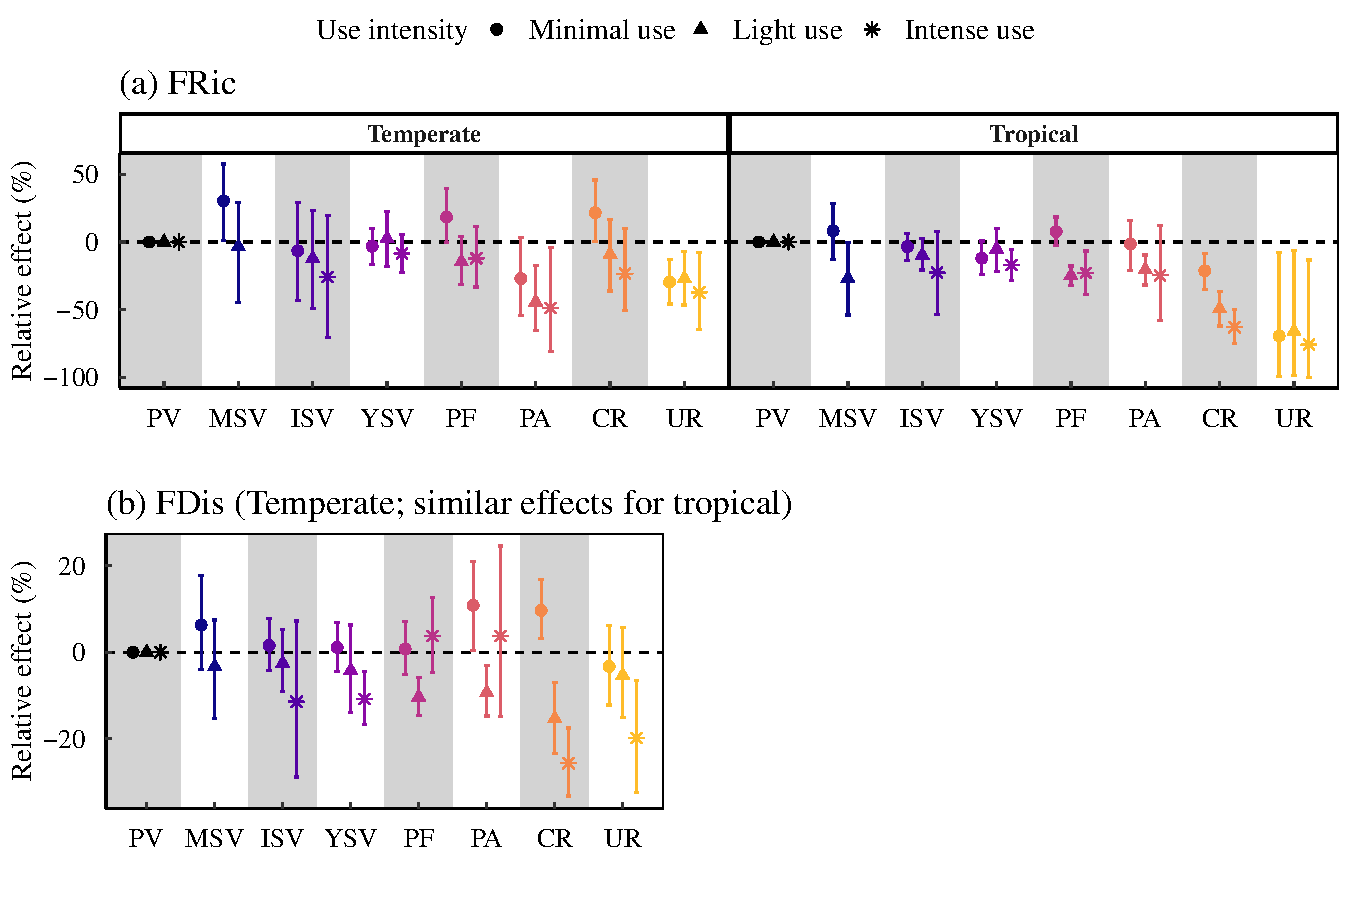
\includegraphics[scale=0.75]{figures/Chapter_FD/Figure2}
\caption[Effects of land use, land-use intensity and region on FRic (a) and on FDis (b) across all PREDICTS vertebrates.]{\textbf{ Effects of land use, land-use intensity and region on FRic (a) and on FDis (b) across all PREDICTS vertebrates.} Effects were rescaled with reference to primary vegetation (PV) and are plotted as a \% difference relative to PV within each land-use intensity. For FRic, the best-fitting model included interactions between land use and region, while these interactions were dropped for FDis, explaining the similar relative effects in both regions. Error bars represent 95\% confidence intervals. MSV: mature secondary vegetation; ISV, intermediate secondary vegetation; YSV, young secondary vegetation; PF, plantation forest; PA, pasture; CR, cropland; UR, urban. Effects for intense use in MSV could not be estimated as there were not enough sampled sites. \textit{Figure reproduced from \citet{Etard2021}.}}
\label{chap3_fig2}
\end{figure}

Fitting the same models to the subset of species with complete trait data, I detected important declines in functional diversity in a number of land uses, showing that the conclusions are robust to trait imputation uncertainty (for example, FRic declined on average by 75\% in intensely used temperate pastoral assemblages; by 48\% for intensely used tropical cropland; and FDis declined by an average 37\% in intensely used tropical urban assemblages; Appendix 2, Figure \ref{SI3_F18}). Furthermore, using the subset of species with complete trait data, I found that the results were not sensitive to the inclusion of geographical range size as an additional trait (Appendix 2, Figure \ref{SI3_F19}). Finally, the results were not sensitive to variation across imputed trait values (Appendix 2, Figure \ref{SI3_F20}) and were also robust to resampling in primary-vegetation sites (Appendix 2, Figure \ref{SI3_F21}).

Responses of FRic and FDis to land use and land-use intensity differed among taxonomic classes (Figure \ref{chap3_fig3}). Within-class effects for FDis were similar between regions. The most notable decreases were observed in lightly- and intensely used agricultural land uses in amphibians, birds and reptiles; and in intensely used urban land uses for birds and mammals. For FRic, the effects in tropical and temperate regions were qualitatively similar in three out of four classes (birds, mammals and reptiles), although effect sizes tended to be bigger for tropical assemblages. Birds and reptiles showed reductions in disturbed land uses in both tropical and temperate regions, whereas I detected few significant effects for mammals. For birds, the most important average decline, of 50\%, was observed in intensely used tropical urban land uses, while for reptiles I detected significant decreases in lightly- and intensely used agricultural sites (but I could not estimate effects for urban land uses due to the small sample size). Finally, the effects differed between tropical and temperate regions for amphibians, with no significant effects detected across temperate assemblages, but important reductions across tropical agricultural and urban assemblages.

%% figure 3
\begin{figure}[h!]
\centering
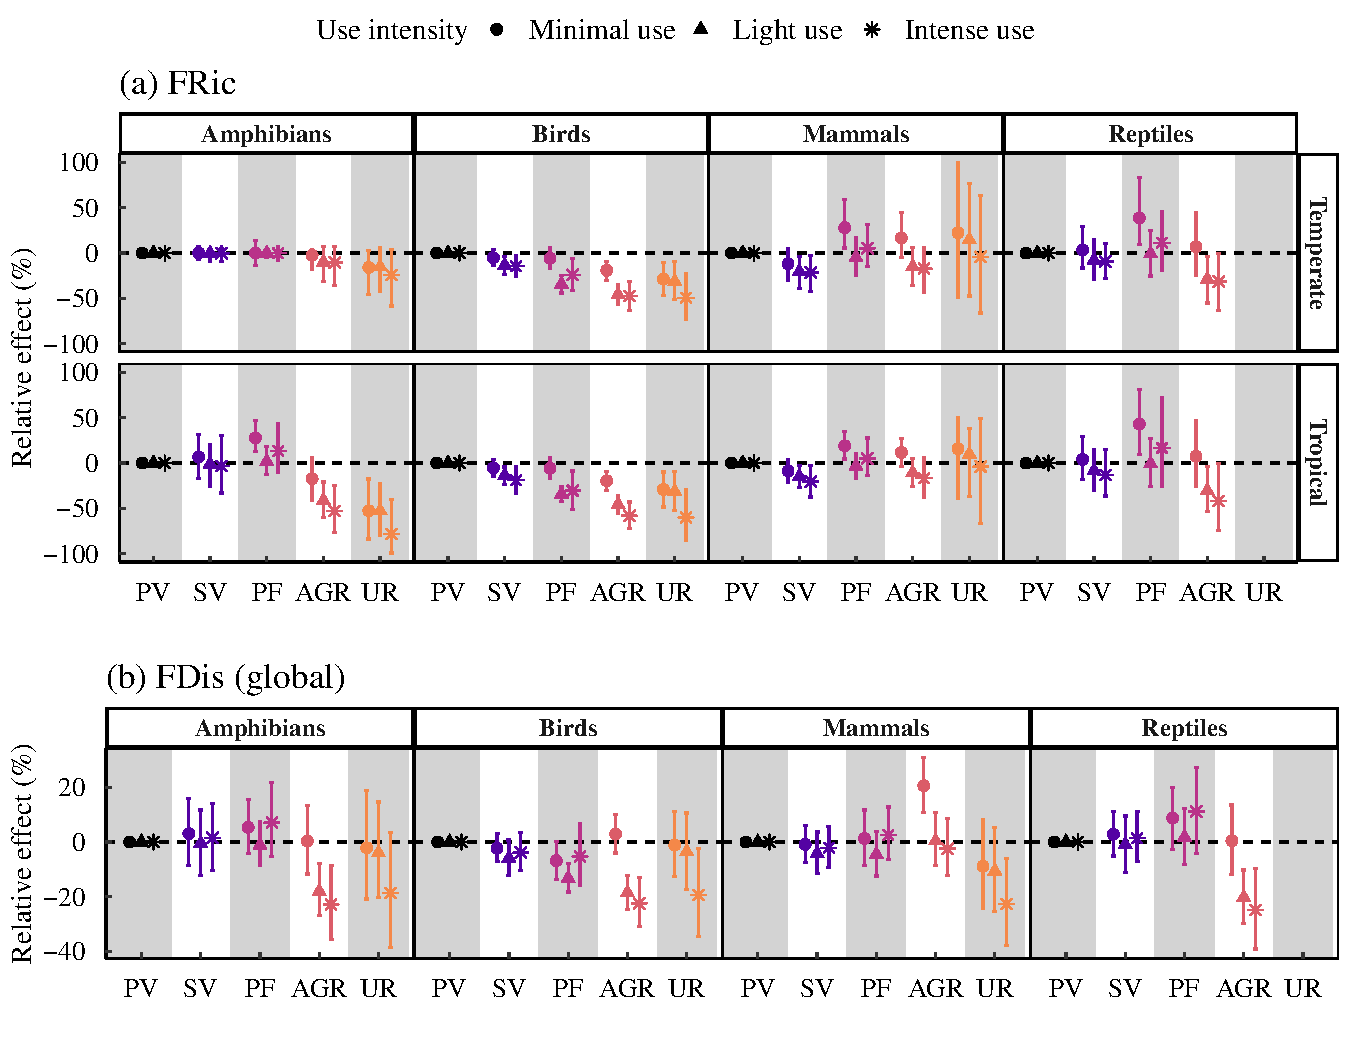
\includegraphics[scale=0.75]{figures/Chapter_FD/Figure3}
\caption[Effects of land use, land-use intensity, region and taxonomic class on FRic (a) and FDis (b).]{\textbf{Effects of land use, land-use intensity, region and taxonomic class on FRic (a) and FDis (b).} Effects were rescaled with reference to primary vegetation (PV) and are plotted as a \% difference relative to PV within each land-use intensity. Error bars represent 95\% confidence intervals. Effects for FRic were estimated from Model 2a, and from Model 2b for FDis. SV, secondary vegetation; PF, plantation forest; AGR, agricultural land uses (pasture and cropland); UR, urban. Effects for reptiles in urban land uses could not be estimated as there were not enough sampled sites. \textit{Figure reproduced from \citet{Etard2021}.}}
\label{chap3_fig3}
\end{figure}

Fitting similar models only for species with complete trait data showed that these patterns are unlikely to be affected by imputation uncertainty for birds; for mammals and reptiles, the main results could even be conservative (Appendix 2, Figures \ref{SI3_F22}, \ref{SI3_F23}). Indeed, although confidence intervals around the estimates were large, I typically observed larger decreases in functional diversity when using the complete data subset, including an 86\% decline in FRic for mammals in intensely used tropical agricultural areas. The results were also unaffected by variation across replicate sets of imputed trait values (Appendix 2, Figure \ref{SI3_F24}).

%\clearpage

\subsection{Changes in the probability of occurrence of functional under-dispersion}

Land use, land-use intensity and region significantly affected the probability of occurrence of functional under-dispersion across vertebrates. Functional under-dispersion was more likely to occur in tropical cropland of all land-use intensities (Figure \ref{chap3_fig4}b), as well as in some of the lightly-used land uses (notably urban and plantation forest). Contrary to my expectations, and with the exception of tropical cropland, functional under-dispersion was not more likely to occur in intensely-used land uses. For minimally-used sites, changes in FDis were mostly consistent with that expected given changes in species richness.

%% figure 4
\begin{figure}[h!]
\centering
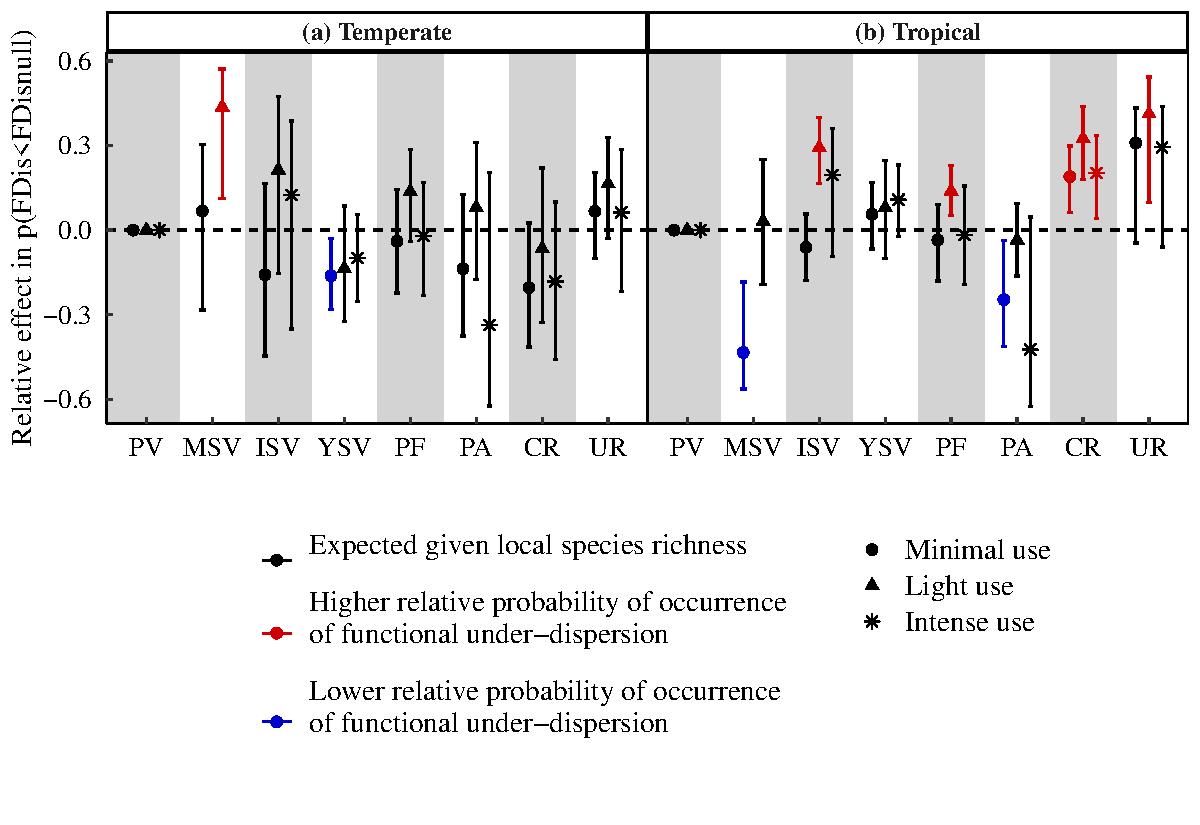
\includegraphics[scale=0.75]{figures/Chapter_FD/Figure4_new}
\caption[Effects of land use, land-use intensity and region on the probability of occurrence of functional under-dispersion.]{\textbf{Effects of land use, land-use intensity and region on the probability of occurrence of functional under-dispersion.} Error bars represent 95\% confidence intervals. PV: primary vegetation; MSV, mature secondary vegetation; ISV, intermediate secondary vegetation; YSV, young secondary vegetation; PF, plantation forest; PA, pasture; CR, cropland; UR, urban. Effects are rescaled and represent the average difference in the probability of occurrence of functional under-dispersion between the reference (PV, probability of functional under-dispersion set at 0 within each land-use intensity) and the disturbed land uses. \textit{Figure reproduced from \citet{Etard2021}.}}
\label{chap3_fig4}
\end{figure}

\subsection{Functional loss and gain}

Across and within vertebrate classes, I detected high levels of functional loss, exceeding the natural turnover between primary-vegetation sites, both in temperate and tropical regions. Across vertebrates (Figure \ref{chap3_fig5}a), functional loss was notably high in temperate pastures (+27\% above reference for minimal use; +73\% for intense use), temperate urban sites (+27\% for light use; +50\% for intense use; effects for tropical urban sites could not be estimated), temperate and tropical cropland (+44\% and +56\% respectively for light use; effects for intense use could not be estimated). Important levels of functional loss were also observed in tropical plantation forest of light use intensity (+51\%; effects for the intense use could not be estimated). High levels of functional loss were also observed within each class (Figure \ref{chap3_fig6}a) (although not all effects could be estimated because of limited sample sizes, Appendix 2, Table \ref{SI3_Table5}). The highest losses were observed in agricultural areas for amphibians and reptiles, with important losses also observed in temperate urban areas for both birds and amphibians (+35\% for minimal use; effects for tropical urban areas could not be estimated).

%% figure 5
\begin{figure}[h!]
\centering
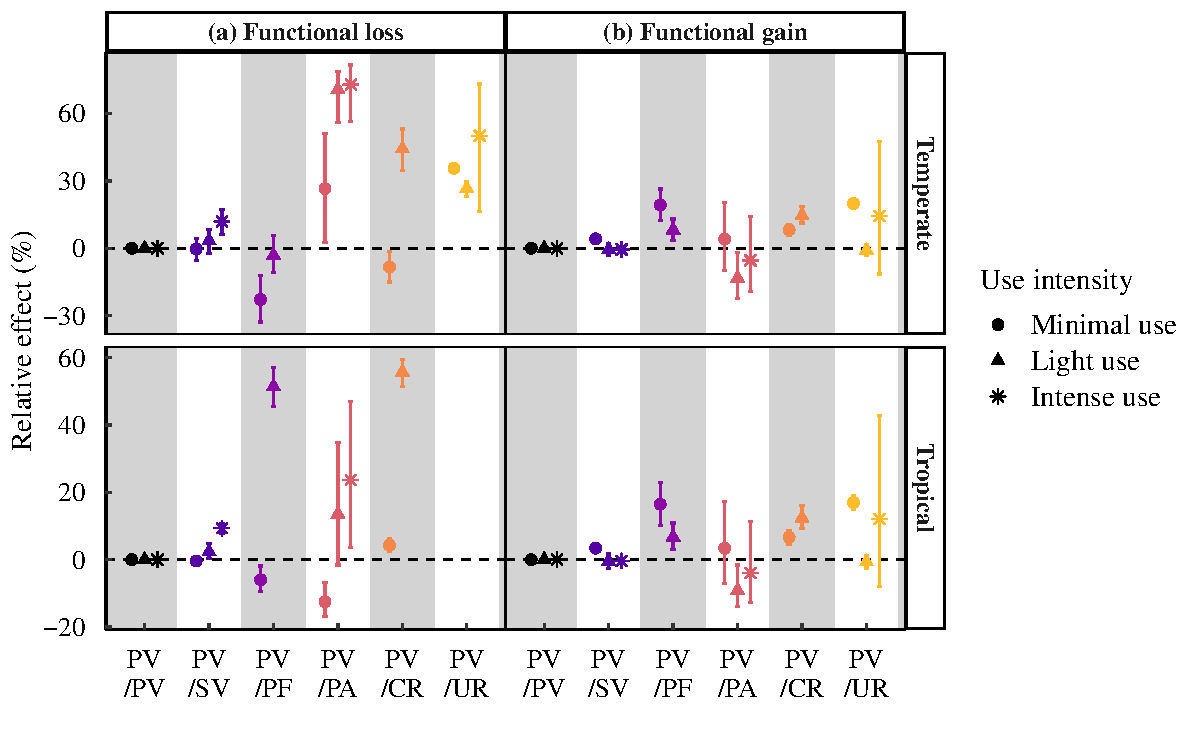
\includegraphics[scale=0.75]{figures/Chapter_FD/Figure5}
\caption[Effects of land use and land-use intensity on (a) functional loss and (b) functional gain across pairs of sites in temperate areas and tropical areas.]{\textbf{Effects of land use and land-use intensity on (a) functional loss and (b) functional gain across pairs of sites in temperate areas and tropical areas.} PV: primary vegetation; SV, secondary vegetation; PF, plantation forest; PA, pasture; CR, cropland; UR, urban. Error bars represent 95\% confidence intervals. Effects are rescaled and represent the average difference in functional loss and gain between the reference pairs (PV/PV, with loss and gain set at 0\% within each land-use intensity), and pairs of primary vegetation with disturbed land uses. Negative effects mean that, on average, levels of functional loss (or gain) were lower than functional loss (or gain) observed between pairs of primary-vegetation sites, and not that there were absolute `negative losses' or `negative gains'. \textit{Figure reproduced from \citet{Etard2021}.}}
\label{chap3_fig5}
\end{figure}

Across vertebrates (Figure \ref{chap3_fig5}b), average functional gain (average proportion of novel trait space in the disturbed assemblage) was moderate and on average did not exceed 20\% in any disturbed land uses. Patterns of functional gain were similar in both regions. The highest functional gains were observed for minimally-used urban sites and plantation forest (range: +16\% to +20\%). On the other hand, important levels of functional gain were observed in some classes (Figure \ref{chap3_fig6}b), with the highest functional gain for mammals (+80\% in intensely used urban sites).

Diagnostic plots (qq-plots and residual distributions) for the models are shown in Appendix 2, Figures \ref{SI3_F9}–\ref{SI3_F17}. Overall, the model residuals were appropriately distributed (but with some leptokurtic residual distributions, to which mixed-effect models are generally robust \citep{Schielzeth2020}).

%% figure 6
\begin{figure}[h!]
\centering
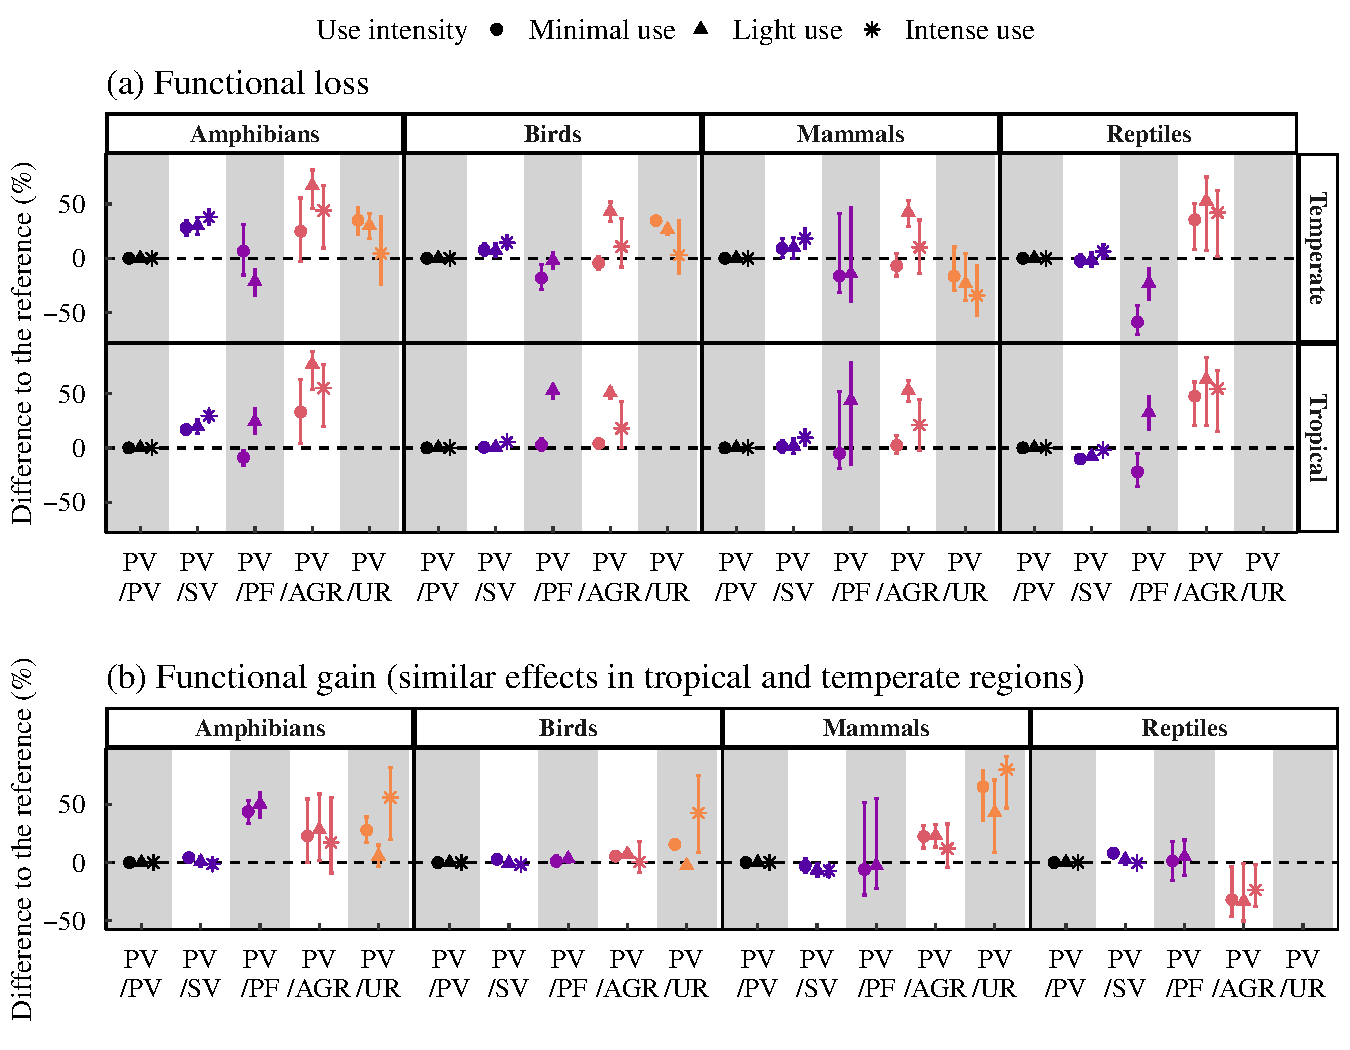
\includegraphics[scale=0.75]{figures/Chapter_FD/Figure6}
\caption[Effects of land use, land-use intensity, region and taxonomic class on functional loss and functional gain across pairs of sites.]{\textbf{Effects of land use, land-use intensity, region and taxonomic class on functional loss and functional gain across pairs of sites.}  PV: primary vegetation; SV, secondary vegetation; PF, plantation forest; AGR, agricultural land uses (pasture and cropland); UR, urban. Error bars represent 95\% confidence intervals. Effects are rescaled and represent the average difference in functional loss and gain between the reference pairs (PV/PV, with loss and gain set at 0\% within each land-use intensity), and pairs of primary vegetation with disturbed land uses. Negative effects mean that, on average, levels of functional loss (or gain) were lower than functional loss (or gain) observed between pairs of primary-vegetation sites, and not that there were absolute `negative losses' or `negative gains'. \textit{Figure reproduced from \citet{Etard2021}.}}
\label{chap3_fig6}
\end{figure}

\clearpage
\section{Discussion}
Here, I showed that the functional diversity of vertebrate assemblages is negatively impacted in human land uses, particularly in the most intensely used land types. The results of this Chapter extend previous studies that have been more taxonomically or geographically restricted \citep{Flynn2009, Matuoka2020}. \citet{Matuoka2020} found that the functional diversity of tropical bird assemblages was negatively affected by human disturbance, a pattern that did not appear in temperate assemblages. Yet, I found that functional diversity was negatively affected in both tropical and temperate areas, with important functional losses in all four vertebrate classes.

Using multiple metrics allowed me to explore different facets of functional diversity. For instance, functional gain could locally offset functional loss in some disturbed land uses. This could indicate that despite no apparent negative effect on FRic, some disturbed land uses (e.g. lightly-used temperate cropland) could experience important functional loss, and highlights the importance of using a variety of indicators. This mechanism could be at play in mammalian assemblages, for which important levels of functional gain were observed in agricultural and urban sites. Further, functional gain in disturbed land uses could indicate that disturbances facilitate the introduction of functionally novel species, falling into previously unoccupied parts of the trait space. This may be because non-native species are more likely to become established in disturbed assemblages. Previous work has shown that land-use disturbance facilitates biological invasions in island ecosystems \citep{Jesse2018,Sanchez-Ortiz2019}, but to my knowledge, this has not been tested specifically across continental areas for invasive vertebrates (but see \citet{Pysek2010}). It is also possible that disturbed areas harbour synanthropic species that do not occur in primary vegetation, leading to substantial functional gain.

Overall, the negative effects of land use on functional richness tended to be more pronounced in the tropics. This is congruent with past studies that have found tropical biodiversity to be disproportionally sensitive to human pressures \citep{Newbold2020, Martins2017}. There are a number of potential explanations for this. First, it could be that a long history of intense land-use disturbance at large scales in many temperate regions (e.g. Western Europe; \citet{Stephens2019}) means that biodiversity is now less sensitive to new disturbances, because the most sensitive species have been filtered out \citep{Balmford1996, Krauss2010, LeProvost2020, Munteanu2020}. Species unable to cope with such disturbances may have gone extinct in the past, while the remaining species would be more disturbance-tolerant \citep{Betts2019}. Tropical regions, historically less disturbed at large scales, would then contain a higher proportion of disturbance-sensitive species than temperate regions. Consequently, the functional richness in undisturbed tropical sites could be less resilient to new disturbances. This also highlights that time since land-use conversion could have important impacts on local functional diversity. Although I did not consider the effects of time since land-use conversion in this work (notably because PREDICTS contained data on time since land-use conversion only for about 22\% of the sites), I expect that time since land-use conversion may affect assemblage composition, and thus, functional diversity, with potentially land-use-specific relationships between time since conversion and functional diversity (e.g., a positive relationship for recovering secondary vegetation or a negative relationship for urban areas; but I did not detect such effects when using the data subset for which there were information on time since land-use conversion [see Appendix 2, S3.8: `Model robustness – time since land-use conversion']).

Second, it could be that tropical species are intrinsically more sensitive to disturbances than temperate species because of their evolutionary history. Natural climatic variability experienced by species as well as species history of exposure to disturbances have been proposed to influence sensitivity to disturbance. For instance, tropical species are, on average, nearer to their climatic limits than temperate species \citep{Deutsch2008, Sunday2014a}. Tropical species could therefore experience more deleterious effects from interacting drivers of change, with land-use change bringing about novel climatic conditions pushing them beyond their tolerance limits \citep{Frishkoff2016, Williams2020a}.

In addition to filtering out sensitive species, land-use change is also expected to modify interactions among species, thereby influencing species persistence \citep{Tylianakis2008, Valiente-Banuet2015}. Although I detected a signal of functional under-dispersion (particularly in tropical cropland), which indicates that assemblages may be locally structured by environment filtering \citep{Bregman2015}, it is likely that several assembly rules underpin assemblage composition \citep{Fournier2016}. For instance, land-use changes could enhance competition among species, promoting over-dispersion by removing species that share similar resources. Such opposite signatures of environmental filtering and enhanced competition on functional dispersion could explain why I did not detect stronger effects of land use on functional under-dispersion occurrence.

Studies looking at impacts of global land use on functional diversity computed with species from all four terrestrial vertebrate classes remain rare. Lack of availability of standardised trait data across terrestrial vertebrates may have hindered such studies from being conducted in the past. To overcome this problem, I based the analyses on a large-scale collation of trait data (Chapter 2; \citet{Etard2020}), and I imputed missing trait values to obtain complete trait datasets in each class. I used random forest algorithms, currently thought to be one of the most robust technique for missing value imputations in trait datasets \citep{Debastiani2021, Johnson2021, Penone2014}. Replicating the analyses on complete trait data subsets showed that imputation uncertainty did not affect the main conclusions of this work and that the negative effects of human land uses were in some cases even stronger when using the complete data subsets. Furthermore, the results were highly consistent across imputed datasets and so insensitive to variation across imputed values. Although missing value imputation can offer a robust filling of missing entries, this study highlights the existing taxonomic biases both in trait data availability and in PREDICTS studies, and thus stresses the need to pursue data compilation efforts, particularly for the least-sampled classes (reptiles and amphibians).

Another implication of trait data availability for vertebrates is that the choice of traits was constrained. \citet{Mouillot2021} showed that functional diversity metrics are sensitive to trait omission and that the sensitivity to trait omission decreases with increasing levels of correlation among traits. Here, I chose seven traits that were available across all classes at least for a subset of the species and that have been implicated in shaping species responses to environmental change. A notable omission was any metric of dispersal ability, which is likely to influence species’ ability to respond to land-use change but is difficult to obtain for most species. In fact, past studies have shown that dispersal abilities can be predicted from ecological correlates, such as body mass, diet or geographical range size \citep{Schloss2012b, Sutherland2000}. Since the results were robust to the omission of geographical range size, I am confident that the omission of dispersal abilities also does not affect the conclusions of this work.

Functional diversity metrics are often used as a proxy for ecosystem functioning because of the conceptual and mechanistic link between functional `effect' traits and ecosystem processes \citep{Lavorel2002a, Violle2007}. In many studies focused on vertebrates, however, functional diversity metrics do not correlate with a given ecosystem function \citep{Hatfield2018}. Here, I did not explicitly target given ecosystem functions, but I argue that evidence of functional loss of vertebrate assemblages indicates that processes sustained by vertebrates are put at risk by land-use change. My results further show that some disturbed land uses are more likely to experience functional under-dispersion, particularly tropical cropland and tropical urban areas, which again indicates a potential imperilment of ecological processes. Indeed, in such cases, decreases in functional dispersion exceed changes expected from the chance removal of species; such non-random modifications indicate that certain areas of the functional trait space are more sensitive to land-use disturbance. Future work could investigate the impacts of land-use change on particular ecosystem functions. The integration of trophic information (beyond the trophic levels I used here) to the species-trait dataset could be an interesting step in that direction, as dietary traits relate to resource use and are, as such, probably the most straightforward traits to link with ecosystem functions. Furthermore, my results suggest that the functional loss experienced within a class is unlikely to be compensated for by the persistence of functionally similar species in other classes. Indeed, I detected negative effects of human land use on functional richness in at least three out of four vertebrate classes (amphibians, birds, and reptiles), in accordance with past studies focusing on each of these groups \citep{Gallmetzer2015, Marcacci2021, Riemann2017, Sol2020}. Although overall mammalian functional richness was less affected, high levels of functional gain suggest that the functional composition of mammalian assemblages is heavily modified in disturbed land uses.

To conclude, the results of this Chapter highlight the negative impacts of human land uses on multiple dimensions of functional diversity, within and across terrestrial vertebrate classes, at a global scale. In many disturbed sites, decreases in functional diversity exceed changes expected from species loss alone, showing that human activities non-randomly reshape ecological assemblages. By intensifying functional loss and promoting functional under-dispersion, land-use change could have deleterious effects on ecosystem functioning, highlighting the necessity of putting into place effective conservation measures in the face of anthropogenic change.